\documentclass[11pt]{ctexart}

% set 1-inch margins in the document
\usepackage[margin=1in]{geometry}
\usepackage{amsthm}
\usepackage{tikz}
\usetikzlibrary{automata}

% include this if you want to import graphics files with /includegraphics
\usepackage{graphicx}
\title{词法分析器之DFA}
\author{宋赟祖}
\begin{document}
	\maketitle
	\begin{enumerate}
		\item 关键字\\
		 auto break case char const continue default\\
		 double else enum extern float for goto in long\\
		 register return short sighed sizeof struct switch
		 typedef union unsigned void volatile while
		
		\item 算术运算符\\
		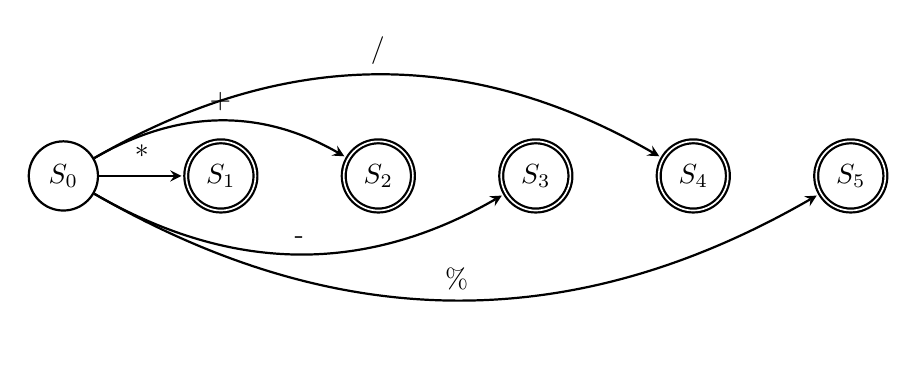
\begin{tikzpicture}[->,>=stealth,shorten >=1pt,auto,node distance=2cm,
		thick,base node/.style={circle,draw,minimum size=12pt}, real node/.style={double,circle,draw,minimum size=35pt}]
		% 算术运算符
		\node[state] (op1) {$S_{0}$};
		\node[state, accepting] (op2) [right of= op1]{$S_{1}$};
		\node[state, accepting] (op3) [right of= op2]{$S_{2}$};
		\node[state, accepting] (op4) [right of= op3]{$S_{3}$};
		\node[state, accepting] (op5) [right of= op4]{$S_{4}$};
		\node[state, accepting] (op6) [right of= op5]{$S_{5}$};
		\path[->]
		(op1) edge node [above] {*} (op2)
		(op1) edge [bend left] node  {+} (op3)
		(op1) edge [bend right] node  {-} (op4)
		(op1) edge [bend left] node  {/} (op5)
		(op1) edge [bend right] node  {\%} (op6);
		\end{tikzpicture}
		
		\item 逻辑运算符 关系运算符\\
		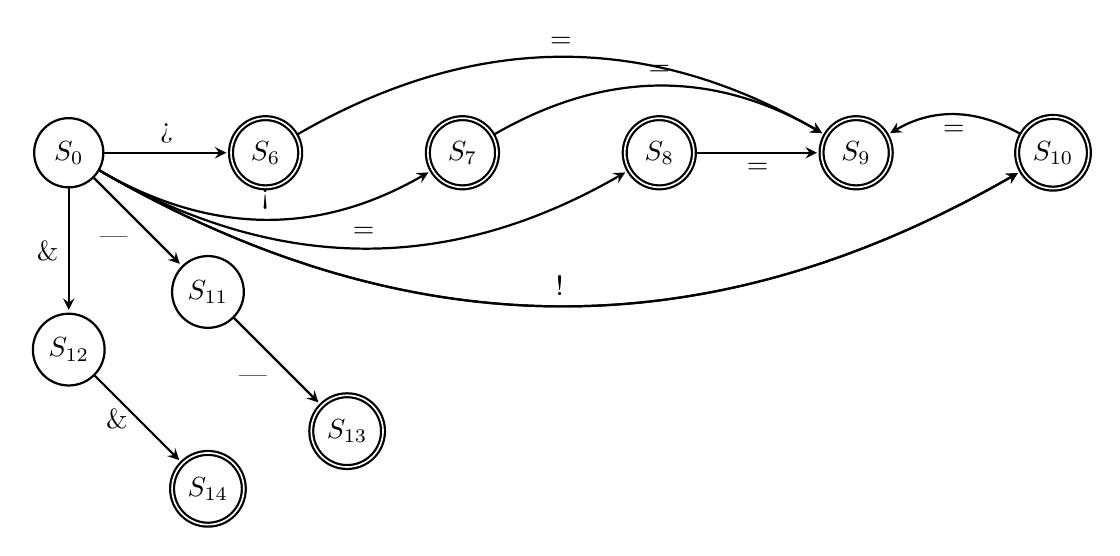
\begin{tikzpicture}[->,>=stealth,shorten >=1pt,auto,node distance=2.5cm,
		thick,base node/.style={circle,draw,minimum size=12pt}, real node/.style={double,circle,draw,minimum size=35pt}]
		% 逻辑运算符
		\node[state] (op7){$S_{0}$};
		\node[state, accepting] (op8) [right of= op7]{$S_{6}$};
		\node[state, accepting] (op9) [right of= op8]{$S_{7}$};
		\node[state, accepting] (op10) [right of= op9]{$S_{8}$};
		\node[state, accepting] (op11) [right of= op10]{$S_{9}$};
		\node[state, accepting] (op12) [right of= op11]{$S_{10}$};
		\node[state] (op13) [below right of= op7]{$S_{11}$};
		\node[state] (op14) [below of= op7]{$S_{12}$};
		\node[state, accepting] (op15) [below right of= op13]{$S_{13}$};
		\node[state, accepting] (op16) [below right of= op14]{$S_{14}$};
		\path[->]
		(op7) edge node [above] {>} (op8)
		(op7) edge [bend right] node  {<} (op9)
		(op7) edge [bend right] node  {=} (op10)
		(op10) edge [below] node  {=} (op11)
		(op7) edge [bend right] node  {!} (op12)
		(op12) edge [bend right] node  {=} (op11)
		(op8) edge [bend left] node  {=} (op11)
		(op9) edge [bend left] node  {=} (op11)
		(op7) edge [bend right] node  {!} (op12)
		(op7) edge [below left] node  {|} (op13)
		(op13) edge [below left] node  {|} (op15)
		(op7) edge [left] node  {\&} (op14)
		(op14) edge [left] node  {\&} (op16);
		\end{tikzpicture}
		
		\item 界符\\
		
		\begin{tikzpicture}[->,>=stealth,shorten >=1pt,auto,node distance=2.5cm,
		thick,base node/.style={circle,draw,minimum size=12pt}, real node/.style={double,circle,draw,minimum size=35pt}]
		% 界符
		\node[state] (b1) [below left of= op16]{$S_{0}$};
		\node[state, accepting] (b2) [right of= b1]{$S_{15}$};
		\node[state, accepting] (b3) [right of= b2]{$S_{16}$};
		\node[state, accepting] (b4) [right of= b3]{$S_{17}$};
		\node[state, accepting] (b5) [right of= b4]{$S_{18}$};
		\node[state, accepting] (b6) [above of= b1]{$S_{19}$};
		\node[state, accepting] (b7) [below of= b1]{$S_{20}$};
		\node[state, accepting] (b8) [above right of= b1]{$S_{21}$};
		\node[state, accepting] (b9) [below right of= b1]{$S_{22}$};
		\node[state, accepting] (b10) [left of= b1]{$S_{23}$};
		\node[state, accepting] (b11) [above left of= b1]{$S_{24}$};
		\node[state, accepting] (b12) [below left of= b1]{$S_{25}$};
		
		\path[->]
		(b1) edge node [above] {;} (b2)
		(b1) edge [bend right] node  {[} (b3)
		(b1) edge [bend left] node  {]} (b4)
		(b1) edge [bend right] node  {.} (b5)
		(b1) edge [left] node  {\}} (b6)
		(b1) edge [left] node  {\{} (b7)
		(b1) edge [left] node  {(} (b8)
		(b1) edge [left] node  {)} (b9)
		(b1) edge [above] node  {,} (b10)
		(b1) edge [above] node  {:} (b11)
		(b1) edge [above] node  {?} (b12);
		\end{tikzpicture}
		
		\item 标识符\\
		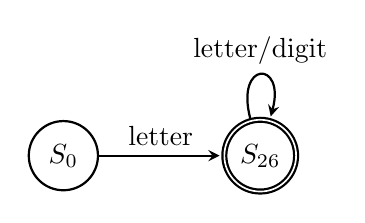
\begin{tikzpicture}[->,>=stealth,shorten >=1pt,auto,node distance=2.5cm,
		thick,base node/.style={circle,draw,minimum size=12pt}, real node/.style={double,circle,draw,minimum size=35pt}]
		% 标识符
		
		\node[state] (id1) {$S_{0}$};
		\node[state, accepting] (id2) [right of= id1]{$S_{26}$};
		\path[->]
		(id1) edge node [above] {letter} (id2)
		(id2) edge [loop above] node  {letter/digit} (id2);
		\end{tikzpicture}
		
		\item 常数\\
		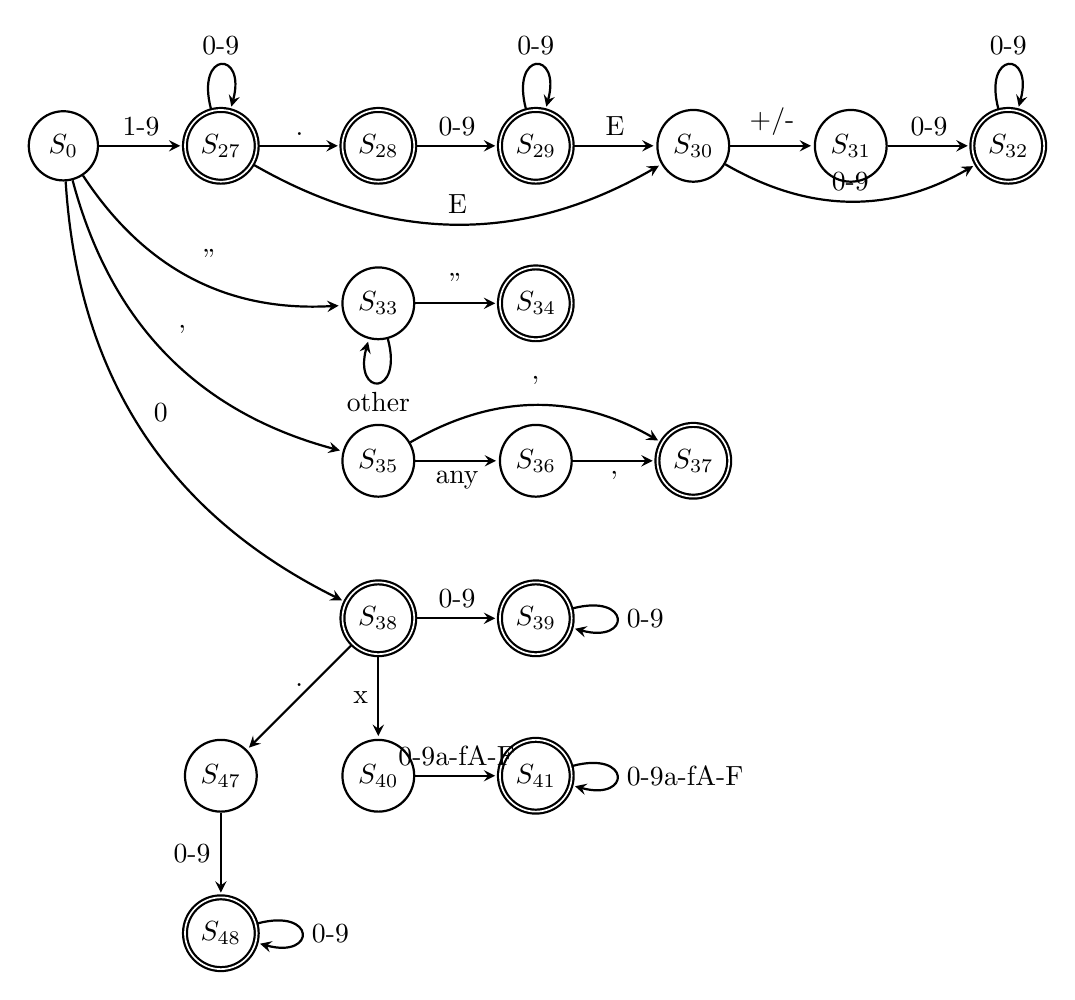
\begin{tikzpicture}[->,>=stealth,shorten >=1pt,auto,node distance=2cm,
		thick,base node/.style={circle,draw,minimum size=12pt}, real node/.style={double,circle,draw,minimum size=35pt}]
		% 常数
		\node[state] (c1) {$S_{0}$};
		\node[state, accepting] (c2) [right of= c1]{$S_{27}$};
		\node[state, accepting] (c3) [right of= c2]{$S_{28}$};
		\node[state, accepting] (c4) [right of= c3]{$S_{29}$};
		\node[state] (c5) [right of= c4]{$S_{30}$};
		\node[state] (c6) [right of= c5]{$S_{31}$};
		\node[state, accepting] (c7) [right of= c6]{$S_{32}$};
		% 字符串常数
		\node[state] (c8) [below of= c3]{$S_{33}$};
		\node[state, accepting] (c11) [right of= c8]{$S_{34}$};
		
		% 字符常数
		\node[state] (c9) [below of= c8]{$S_{35}$};
		\node[state] (c12) [right of= c9]{$S_{36}$};
		\node[state, accepting] (c13) [right of= c12]{$S_{37}$};
		
		% 八进制常数 十六进制常数
		\node[state, accepting] (c10) [below of= c9]{$S_{38}$};
		\node[state, accepting] (c14) [right of= c10]{$S_{39}$};
		\node[state] (c15) [below of= c10]{$S_{40}$};
		\node[state, accepting] (c16) [right of= c15]{$S_{41}$};
		
		% 小数
		\node[state] (c17) [left of= c15]{$S_{47}$};
		\node[state, accepting] (c18) [below of= c17]{$S_{48}$};
		
		
		\path[->]
		(c1) edge node [above] {1-9} (c2)
		(c2) edge [loop above] node  {0-9} (c2)
		(c2) edge [above] node  {.} (c3)
		(c3) edge [above] node  {0-9} (c4)
		(c4) edge [loop above] node  {0-9} (c4)
		(c4) edge [above] node  {E} (c5)
		(c2) edge [bend right] node  {E} (c5)
		(c5) edge [above] node  {+/-} (c6)
		(c5) edge [bend right] node  {0-9} (c7)
		(c6) edge [above] node  {0-9} (c7)
		(c7) edge [loop above] node  {0-9} (c7)
		
		% 字符串
		(c1) edge [bend right] node  {"} (c8)
		(c8) edge [loop below] node  {other} (c8)
		(c8) edge [above] node  {"} (c11)
		
		
		% 字符常数
		(c1) edge [bend right] node  {'} (c9)
		(c9) edge [below] node  {any} (c12)
		(c12) edge [below] node  {'} (c13)
		(c9) edge [bend left] node  {'} (c13)
		
		% 八进制
		(c1) edge [bend right] node  {0} (c10)
		(c10) edge [above] node  {0-9} (c14)
		(c10) edge [left] node  {x} (c15)
		(c14) edge [loop right] node  {0-9} (c14)
		(c15) edge [above] node  {0-9a-fA-F} (c16)
		(c16) edge [loop right] node  {0-9a-fA-F} (c16)
		
		% 小数
		(c10) edge [above] node  {.} (c17)
		(c17) edge [left] node  {0-9} (c18)
		(c18) edge [loop right] node  {0-9} (c18);
		
		
		
		\end{tikzpicture}
	
		
		\item 注释 \\
		% 注释
		\begin{tikzpicture}[->,>=stealth,shorten >=1pt,auto,node distance=2cm,
		thick,base node/.style={circle,draw,minimum size=12pt}, real node/.style={double,circle,draw,minimum size=35pt}]
		\node[state] (com1) {$S_{0}$};
		\node[state] (com2) [right of= com1]{$S_{42}$};
		\node[state] (com3) [right of= com2]{$S_{43}$};
		\node[state] (com4) [right of= com3]{$S_{44}$};
		\node[state, accepting] (com5) [right of= com4]{$S_{45}$};
		\path[->]
		(com1) edge node [above] {/} (com2)
		(com2) edge [above] node  {*} (com3)
		(com3) edge [loop above] node  {other} (com3)
		(com3) edge [above] node  {*} (com4)
		(com4) edge [bend left] node  {other} (com3)
		(com4) edge [loop above] node  {*} (com4)
		(com4) edge [above] node  {/} (c5);
		\end{tikzpicture}
		
		\item 空白 \\
		% 空白
		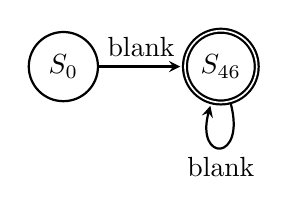
\begin{tikzpicture}[->,>=stealth,shorten >=1pt,auto,node distance=2cm,
		thick,base node/.style={circle,draw,minimum size=12pt}, real node/.style={double,circle,draw,minimum size=35pt}]
		\node[state] (bk1) {$S_{0}$};
		\node[state, accepting] (bk2) [right of= bk1]{$S_{46}$};
		\path[->]
		(bk1) edge node [above] {blank} (bk2)
		(bk2) edge [loop below] node  {blank} (bk3);
		\end{tikzpicture}
		
		
	\end{enumerate}
		
\end{document}

